\documentclass[addpoints]{exam}

%These tell TeX which packages to use.
\usepackage{array,epsfig}
\usepackage{amsmath}
\usepackage{amsfonts}
\usepackage{amssymb}
\usepackage{amsxtra}
\usepackage{amsthm}
\usepackage{mlextra} % must be below ams packages
\usepackage{mathrsfs}
\usepackage{color}
\usepackage{array}
\usepackage{graphicx}
\graphicspath{ {../art/} }
\usepackage{bm}
\usepackage{tikz}
\usepackage{multicol}

%Pagination stuff.
\setlength{\topmargin}{-.3 in}
\setlength{\oddsidemargin}{0in}
\setlength{\evensidemargin}{0in}
\setlength{\textheight}{9.in}
\setlength{\textwidth}{6.5in}



\newcommand{\twonode}{%
  \begingroup\normalfont
  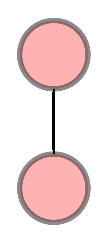
\includegraphics[height=\fontcharht\font`\b]{2nodetree.eps}%
  \endgroup
}


\begin{document}


\noindent
%\begin{tabular*}{\textwidth}{l @{\extracolsep{\fill}} r @{\extracolsep{6pt}} l}
%	{\large CS3920: Foundations of Computer Science} &  \makebox[3in]{\large Name:\enspace\hrulefill}\\
	%{Points: /\numpoints\. } \\
	%{\large June 8, 2018} & \\
%	{\large Quiz 2} & \\
%	{\large Points: \hspace{1cm}/\numpoints} & 
%\end{tabular*}\\

%\fbox{\fbox{\parbox{6in}{\textbf{Instructions}: Please answer the questions 
%			below to the best of your ability. Be sure to show your work where appropriate. 
%			This quiz is closed book, closed notes, closed computer.}}}\\

\begin{center}
{\LARGE	Resolution Exercises}
\end{center}

\vspace{1cm}

\begin{questions}
	
\question 
Consider the following set of formulas $A$ shown in clausal form.

 $\{p, \bar{p}q, p\bar{q}, \bar{p}\bar{q} \}$ \\
 
\begin{parts}
\part Refute using resolution.

\vspace{4cm}
	



\part Write $A$ as a single formula in CNF. 

What can you say about $ \lnot (p \land (\lnot p \lor q) \land (p \lor \lnot q) \land (\lnot p \lor \lnot q))$ ?
	\end{parts}

\vspace{3cm}	
	
\question Transform the following set of formulas to clausal form and refute using resolution.

$\{p, p \rightarrow ((q \lor r) \land \lnot (q \land r), p \rightarrow ((s \lor t) \land \lnot (s \land t), s \rightarrow q, \lnot r \rightarrow t, t\rightarrow s \}$ 








\end{questions}
\end{document}


